% !TeX encoding = UTF-8
% !Tex spellcheck = de_DE

%begin:Silbentrennung ****
\RequirePackage{hyphsubst}
\HyphSubstIfExists{ngerman-x-latest}{\HyphSubstLet{ngerman}{ngerman-x-latest}}{} 
\listfiles
%end:Silbentrennung ******

\documentclass[12pt,a4paper]{article}
% ***********************************************************
% ***************** MyStyle - Rene Vollmer*******************
% ***********************************************************
% Version 1.0b



\usepackage[utf8]{inputenc}

\usepackage{hyperref}

\usepackage{amsmath} % AMS Math Package
\usepackage{amsfonts}
\usepackage{amsthm} % Theorem Formatting
\usepackage{amssymb}	% Math symbols such as \mathbb
\usepackage{mathtools}
\usepackage{graphicx} % Allows for eps images
\usepackage{multicol} % Allows for multiple columns
\usepackage[]{units}

\usepackage{hyperref} %Links
\usepackage{url}

\usepackage{verbatim} %Fuer mehrzeilige kommentare \begin{comment} \end{comment}

%\usepackage[table]{xcolor}
\usepackage{array,ragged2e}

\usepackage[hang]{caption} % Captions einrücken
\usepackage{subfigure}
%\usepackage{subfig}

%Some other shit
\usepackage{float}
%\floatstyle{boxed} %Puts a box around each figure
\restylefloat{figure}
%\usepackage{wrapfig}
\usepackage{microtype}



\usepackage{xparse} % For uses like \DeclareDocumentCommand{\foocmd}{ O{default1} O{default2} m }{#1~#2~#3}


\usepackage{color}
\definecolor{gray}{rgb}{.5,.5,.5}
\definecolor{lightgray}{rgb}{.25,.25,.25}

%Graphics (PGF / TIKZ) **+**+**+**+**+**+**+**+**+**+**+**+**+**+
\usepackage{tikz}
\usetikzlibrary{patterns}
\tikzset{
	hatchhor/.style={pattern=horizontal lines,pattern color=#1},
	hatchhor/.default=black
}
\tikzset{
	hatchvert/.style={pattern=vertical lines,pattern color=#1},
	hatchvert/.default=black
}
\tikzset{
	hatchdiag/.style={pattern=north east lines,pattern color=#1},
	hatchdiag/.default=black
}
\tikzset{
	hatchdiag2/.style={pattern=north west lines,pattern color=#1},
	hatchdiag2/.default=black
}
%also possible grid, crosshatch, dots, crosshatch dots, fivepointed stars, sixpointed stars

\usepackage{pgfplots}
\usepgfplotslibrary{fillbetween}

% Style to select only points from #1 to #2 (inclusive)
\pgfplotsset{select coords between index/.style 2 args={
		x filter/.code={
			\ifnum\coordindex<#1\def\pgfmathresult{}\fi
			\ifnum\coordindex>#2\def\pgfmathresult{}\fi
		}
	}
}


\newcommand{\vasymptote}[2][]{
	\draw [color=gray,densely dashed,#1] ({rel axis cs:0,0} -| {axis cs:#2,0}) -- ({rel axis cs:0,1} -| {axis cs:#2,0});
}

\newcommand{\vertline}[2][]{
	\draw [#1] ({rel axis cs:0,0} -| {axis cs:#2,0}) -- ({rel axis cs:0,1} -| {axis cs:#2,0});
}
%END Graphics **+**+**+**+**+**+**+**+**+**+**+**+**+**+**+**+**+

\input{style/newsymbols.tex}


% ******************************~~~~*****************************
%Photo quality management. This is an old try:
\newcommand\openfile{\newwrite\outputstream\immediate\openout\outputstream=photo.log
	\writetofile[linewidth]{\the\linewidth}
	\writetofile[textwidth]{\the\textwidth}
	\writetofile[dpi]{300}
	}
\newcommand\closefile{\immediate\closeout\outputstream}
\newcommand\writetofile[2][2]{\immediate\write\outputstream{#1 #2}}

\newcommand\photo[2][2]{\includegraphics[width=#1]{#2}\writetofile[#2]{#1}}

% ***************************************************************
% And this is working
% Reduce image size for fixed dpi
% Introduce \includegraphicsRS for this purpose

% for downsampling large images: \includegraphicsRS
% (\includegraphics "resize")
% \includegraphicsRS[#1][#2]{#3}
% #1 = normal \includegraphics[] - Parameter (like scale=1) {optional}
% #2 = approx part of the screen, eg half page width use 0.5 or 1/2 {optional}
%      reduces to #2*1000px
% #3 = relative path to image file WITH ending (e.g. .jpg) {required}
\pdfimageresolution 300

\newcommand{\includegraphicsRS}{}

\ifnum\pdfshellescape=1
% Yes, enabled
% IFP - image file path
% IFN - image filename only
% here resizing at #2*1000 px wide
\newread\myinput
% must add default argument [] so typeout works
\DeclareDocumentCommand{\includegraphicsRS}{ O{\@empty} O{1} m }{ %
%\renewcommand\includegraphicsRS[2][\@empty]{
	% run downsampling bash script
	\immediate\write18{mkdir -p images; mkdir -p images/downsampled; IFP=#3 ; %
		PIX=#2 ; PIX=$( awk  'BEGIN { rounded = sprintf("\%.0f", ('$PIX')*1000); print rounded }' ) ;
		echo "$PIX 1000 *p" | dc ; %
		echo "Processing $IFP" ; %
		IFN=$(basename $IFP) ; %
		echo "images/downsampled/$IFN" > tmpname ; %
		if [ ! -f images/downsampled/$IFN ]; then %
		echo "File images/downsampled/$IFN not found! Converting..." ; %
		%the \string> after the pixel width (e.g. 1000x) will prevent imagemagick from producing files larger than the original
		convert $IFP -resize $PIX"x\string>" -quality 85 images/downsampled/$IFN ; %

		else %
		echo "Found images/downsampled/$IFN - reusing." ; %
		fi ; %
		%alternatively: bash includegraphicsRS.sh #3 #2
		%and have the code in the *.sh-file.
	} % end write18
	% here we should have downsampled file
	% retrieve downsample filename first
	\immediate\openin\myinput=tmpname
	% The group localizes the change to \endlinechar
	\bgroup
	\endlinechar=-1
	\immediate\read\myinput to \localline
	% Since everything in the group is local, we have to explicitly make the
	% assignment global
	\global\let\myTmpFileName\localline
	\egroup
	\immediate\closein\myinput
	% Clean up after ourselves
	% \immediate\write18{rm -f -- tmpname}
	% finally, include downsampled image
	\includegraphics[#1]{\myTmpFileName}
} % end renewcommand
\else
% No, disabled
% in this case, \includegraphicsRS is just the usual \includegraphics
\renewcommand\includegraphicsRS[2][\@empty]{%
	\includegraphics[#1]{#2}
}
\fi

\begin{comment}
old stuff, not used any longer. Could be useful for future changes though.
\usepackage{fp}

\newlength{\TOarg} \newlength{\TOunit}
{\catcode`p=12 \catcode`t=12 \gdef\TOnum#1pt{#1}}
\newcommand\TOop[2]{\setlength{\TOarg}{#2}%
	\FPdiv\TOres{\expandafter\TOnum\the\TOarg}{\expandafter\TOnum\the\TOunit}%
	\FPround\TOres\TOres{#1}}
\newcommand{\TOspace}{\ }
\newcommand\TOpt[2][2]{\setlength{\TOunit}{1pt}\TOop{#1}{#2}\TOres\TOspace pt}
\newcommand\TOin[2][2]{\setlength{\TOunit}{1in}\TOop{#1}{#2}\TOres\TOspace in}
\newcommand\TOcm[2][2]{\setlength{\TOunit}{1cm}\TOop{#1}{#2}\TOres\TOspace cm}
\newcommand\TOmm[2][2]{\setlength{\TOunit}{1mm}\TOop{#1}{#2}\TOres\TOspace mm}
\newcommand\TOem[2][2]{\setlength{\TOunit}{1em}\TOop{#1}{#2}\TOres\TOspace em}
\newcommand\TOpx[2][2]{\setlength{\TOunit}{1px}\TOop{#1}{#2}\TOres\TOspace px}
\newcommand\TOptdeux[2][2]{\setlength{\TOunit}{1pt}\TOop{#1}{#2}\TOres}

convert $IFP -resize 50\% images/downsampled/$IFN ; %		textwidth="\the\textwidth" ; %
TW=${textwidth:0:(-2)} ; %
VARI="$TW"; %
convert -resize 2000x -units pixelspercentimeter $IFP -density 120 -pointsize 30 -draw "gravity south-east fill black text 0,5 '$VARI'" downsampled/$IFN ; %
\end{comment}


% END of \includegraphicsRS
% ***************************************************************
% ******************************~~~~*****************************



% ***********************************************************
% ********************** END HEADER *************************
% ***********************************************************
\usepackage[left=2.50cm, right=2.50cm, top=2.50cm, bottom=2.00cm]{geometry}


\usepackage[ngerman]{babel}

%test
\begin{comment}
\usepackage{titlesec}
\titleformat{\subsection}[runin]% runin puts it in the same paragraph
{\normalfont\bfseries}% formatting commands to apply to the whole heading
{\thesubsection}% the label and number
{0.5em}% space between label/number and subsection title
{}% formatting commands applied just to subsection title
[]% e.g. [.] punctuation or other commands following subsection title\frac{•}{•}
\end{comment}

\linespread{1.1}
\usepackage{microtype}

%\addto\captionsgerman{ \renewcommand{\figurename}{\small{\textbf{Abb.}}}
%\captionsetup{figurewithin = section}
%\captionsetup{font=small, labelfont=bf} }


\begin{document}
	
	\pagenumbering{Roman}
	%TODO REMOVE
	%\textbf{TODO}
	%
René
\begin{enumerate}
	\item Regina sagen, dass sie auf die Eigenschaften der FT refen soll
	\item Regine Videos vom Handy geben
	\item Regina Rücktransformierte Bilder geben
	\item 
\end{enumerate}

Vivi
\begin{enumerate}
	\item ...
	\item ...
\end{enumerate}
	
	
	%Metadaten
	\title{\textit{Fortgeschrittenenpraktikum}\\\textbf{Optische Fouriertransformation} }
	\date{August 2015}
	\author{Vivien Sleziona \footnote{vivi.s@arcor.de}\\ Regina Schauer \footnote{regina.schauer@web.de}\\ René Vollmer \footnote{rene.vollmer@studium.uni-hamburg.de} \\ \\Betreut durch\\ Kai Morgener\footnote{kmorgene@physnet.uni-hamburg.de}}
	
	\maketitle
	
	\begin{center} 
		\bigskip
		\bigskip
		
		\begin{minipage}{0.75\textwidth}
			\textbf{[Zusammenfassung]}
			% !TeX root = ../praktikum.tex
% !TeX encoding = UTF-8
% !Tex spellcheck = de_DE

Die Fourier-Analytik und insbesondere die Fouriertransformation sind auf vielen modernen Anwendungen kaum noch weg zu denken. Sie ist essentieller Bestandteil vieler Bildverarbeitungsalgorithmen \cite{easton_fourier_2010} und -kompressionsverfahren wie JPEG \cite{_jpeg_2015}, sie wird genutzt um Bildinformationen Computeralgorithmen zugänglich zu machen \cite{prof._dr._norbert_link_vorlesungsscript:_????} und in vielen anderen Bereichen der Signalverarbeitung. Weitere Anwendungen liefert das Schlierenverfahren, z.B. in der Luftfahrt oder bei der Motorenentwicklung, da mit diesem Gas- und Flüssigkeitsströmungen sichtbar gemacht werden können.\\

In diesem Versuch wird mit einfachen optischen Mitteln eine Fouriertransformation an Bildern durchgeführt und die Fouriertransformierte manipuliert. Dabei wird dem Leser ein intuitives Verständnis für die Funktionsweise und Bedeutung von Fouriertransformationen vermittelt.
		\end{minipage}
	\end{center}
	
	%\vfill
	\newpage
	
	\tableofcontents
	\vfill
	\newpage
	\clearpage	
	
	\pagenumbering{arabic}
	
	\section{Theoretische Grundlagen}
	% !TeX root = ../praktikum.tex
% !TeX encoding = UTF-8
% !Tex spellcheck = de_DE

\subsection{Zweidimensionales Elektronengas}

Damit es zum Quanten-Hall-Effekt kommen kann, müssen einige Bedingungen erfüllt sein. Eine davon ist die Existenz eines zweidimensionalen Elektronengases.
In einem zweidimensionalen Elektronengas (2DEG) ist die Bewegung der freien Elektronen auf eine Ebene eingeschränkt. Es gibt verschiedene Möglichkeiten dies zu erreichen. 
\subsubsection{Aufbau der Probe}
In diesem Versuch wird dazu eine AlGaAs-GaAs-Heterostruktur verwendet, siehe Abbildung \ref{fig:Proben_Aufbau}. Die darin gestapelten, unterschiedlichen, einkristallinen Halbleitermaterialien sorgen aufgrund ihrer verschiedenen Bandlücken dafür, dass der Verlauf der Leitungs- bzw. Valenzbandkante in Stapelrichtung einen sehr kleinen Potentialtopf für die Leitungsbandelektronen erzeugt. Der elektronische Transport ist so in Stapelrichtung stark eingeschränkt, während sich die Elektronen in den anderen beiden Raumrichtungen bewegen können. Dabei muss die Bandverbiegung so sein, dass der Bereich des Potentialtopfes nur wenige Nanometer zwischen den Schichten einnimmt.

\begin{figure}[h]
\centering
\includegraphics[width=0.7\linewidth]{images/Anleitungsheft/2DEG_Anleitungsheft}
\caption[2DEG Schicht]{vereinfachter Aufbau der GaAs-AlGaAs-Heterostruktur}
\label{fig:Proben_Aufbau}
\end{figure}

In Abbildung \ref{fig:Proben_Aufbau} ist der schematische Aufbau der in diesem Experiment untersuchten Probe dargestellt. 
Während sich die Gitterkonstanten der beiden Materialen um weniger als ein Prozent unterscheiden, liegt die Bandlücke des  Silizium-dotierten GaAs  höher als die des GaAs, sodass das Leitungsband des GaAs energetisch günstigere Zustände besitzt. Daher kommt es zum Elektronenfluss aus dem AlGaAs in das undotierte GaAs und so zu einem Verbiegen des Leitungs- und Valenzbandes, dargestellt in Abbildung \ref{fig:Proben_Aufbau}, rechts.
Der näherungsweise Potentialtopf, welcher sich im Leitungsband zwischen dem AlGaAs und dem GaAs ausbildet, besitzt ein Minimum unterhalb der Fermienergie $E_F$ und aufgrund seiner energetisch günstigeren Lage, werden die Elektronen in diesem Potentialtopf gefangen. 
In der Abbildung wird das AlGaAs auch als Spacer bezeichnet, denn diese Schicht in der Probe dient hauptsächlich dazu, Streupotentiale zwischen GaAs und der Dotierschicht AlGaAs:Si zu reduzieren, um die mittlere freie Weglänge und damit die Beweglichkeit der Elektronen zu erhöhen. Die Deckschicht GaAs:Si dient lediglich zum Schutz der Probe vor Oxidation und hat keine technische Bedeutung.

\subsubsection{Quantenmechanische Beschreibung unter Einfluss eines Magnetfeldes}
In der quantenmechanischen Beschreibung des 2DEGs findet man für die Energien der Elektronen aufgrund der Einschränkung ihrer Bewegung in z-Richtung quantisierte Werte. $E_z$ nimmt die Werte i mit i = 1, 2, 3, ... an, während die Bewegung der Elektronen in x- und y-Richtung uneingeschränkt bleibt.So setzt sich die Energie der Elektronen wie folgt zusammen:

\begin{equation}
E(k_x,k_y,i)=\frac{\hbar^2k_x^2}{2m^*}+\frac{\hbar^2k_y^2}{2m^*}+E_i^z   \text{~~~~~~~~~ mit ~~~} i=1,2,3....
\label{eq:energie_2DEG}
\end{equation}

Hier sind $k_x$ und $k_y$ die Wellenvektoren der Elektronen in $x -$ und $y-$ Richtung und $m^*$ ist die effektive Masse. $i = 1,2,3...$  entspricht der Quantisierung in $z-$ Richtung, welche zur Folge hat, dass sich für jedes Energieniveau ein zweidimensionales  Leitungsband in $x-$ und in $y-$ Richtung ausbildet. 
Es ist für das hier durchgeführte Experiment zum Quanten-Hall-Effekt essentiell, die Energierelationen der Elektronen im zweidimensionalen Elektronengas zu bestimmen. 

Die Zustandsdichte D in einem Band ergibt sich aus der Anzahl der Elektronenzustände $N$ pro Energieintervall und Probenvolumen $V$ und kann mit Gleichung~\eqref{eq:energie_2DEG} geschrieben werden als:

\begin{equation}
	D(E)=\frac{1}{V}\d{N(E)}{E}=g\frac{m^*}{2\pi\hbar^2}
	\label{eq:2DEG_zustandsdich} 
\end{equation}

Mit dem Probenvolumen V und der Teilchenzahl N. Der rechte Term folgt dabei aus der Zweidimensionalität des Probenvolumens und aus Gleichung \ref{eq:energie_2DEG}.
Die Zustandsdichte D(E) in dem Leitungsband eines 2DEGs ist also konstant mit dem Entartungsfaktor g. Für die Spinentartung ist $g_s=2$. Im senkrechten Magnetfeld ist die Bewegung der Elektronen auch in der xy-Ebene festgelegt.

Wenn nun ein Magnetfeld angelegt wird, werden die freien Elektronen klassisch durch die Lorentz-Kraft auf Kreisbahnen abgelenkt. Diese lässt sich durch die Überlagerung zweier senkrecht aufeinander stehenden harmonischen Schwingungen beschreiben, die senkrecht zueinander in der xy-Ebene schwingen. Der Abstand der Energiewerte ist durch $\hbar \omega_c$ gegeben,
mit der Kreisfrequenz:

\begin{equation}
\omega_c=\frac{eB}{m^*}
\label{eq:kreisfrequenz}
\end{equation}

Diese Kreisfrequenz wird auch Zyklotronfrequenz genannt. Da die Energieniveaus eines solchen Oszillators äquidistant sind, folgt für die Elektronenenergiedispersion des 2DEG in einem in z-Richtung angelegten Magnetfeld

\begin{equation}
E=E_i^z +(n+\frac{1}{2})\hbar\omega_c +g_L^*\mu_B Bs \text{~~~~~~~~~~mit~~~~~} n,i=1,2,3...
\label{eq:elektr_disp_bfeld}	
\end{equation}

Mit dem effektiven Lande-Faktor $g^*_L$, dem bohrschen Magneton $\mu_B$ und der Spinquantenzahl $s=\nicefrac{+}{-}\frac{1}{2}$.
Die Energien $E_n$ heißen Landau-Niveaus. Der mittlere Term der Gleichung beschreibt die kinetische Energie der Elektronen
in quantenmechanischer Betrachtung und der rechte Term berücksichtigt die Spin-Bahn-Wechselwirkung des Systems. 

\begin{figure}[h]
\centering
\includegraphics[width=0.7\linewidth]{images/Anleitungsheft/Landauniveaus_Anleitungsheft}
\caption[Landau Niveaus]{Vergleich der klassischen Beschreibung der Energieabhängigkeit (a) mit der Quantenmechanischen (b). (c) Vergleich des Zusammenhanges zwischen Zustandsdichte und Energie in klassischer und quantenmechanischer Beschreibung.}
\label{fig:Landauniveaus_Anleitungsheft}
\end{figure}

Abbildung \ref{fig:Landauniveaus_Anleitungsheft} veranschaulicht das Annehmen diskreter Werte der Zustandsdichte im quantenmechanischen Fall. 
Das Magnetfeld wirkt auf die Bewegungsrichtung der Elektronen, nicht aber auf deren kinetische Enegie, daher lässt sich die Anzahl der Elektronen pro Zustand mit der Zustandsdichte $D(E)$ bei $B=\unit[0]{T}$ ausdrücken mit

\begin{equation}
N_L=\frac{D(E)}{g}\hbar\omega_c = \frac{eB}{h}
\label{eq:zustandsd_pro_landauniveau}
\end{equation}

Daraus ist ersichtlich, dass die Anzahl der Elektronen pro Flächeneinheit, die ein Landauniveau aufnehmen kann, linear mit dem Magnetfeld zunimmt. Es wird ein Füllfaktor $\nu$ eingeführt, welcher angibt, wie viele Spin aufgespaltenen Landau-Niveaus bei gegebener Ladungsträgerdichte $n_s$ und einem Magnetfeld B zumindest teilweise besetzt sind:

\begin{equation}
\nu=\frac{n_s}{N_L}=\frac{hn_s}{eB}
\label{eq:einfuehrung_fuellfakt}
\end{equation}

\newpage
\subsection{Klassischer Hall-Effekt}

Beim klassischen Hall-Effekt liegt ein Magnetfeld B senkrecht zu einem stromdurchflossenen Leiter an. Das Magnetfeld wirkt durch die Lorentzkraft auf die bewegten Ladungsträger und es bildet sich die sogenannte Hallspannung $U_{Hall}$ senkrecht zur Strom- und Magnetfeldrichtung aus. Die Hallspannung ist proportional zum angelegten Magnetfeld. Dieser Effekt wurde 1879 von dem amerikanischen Physiker Edwin H. Hall entdeckt.

\begin{figure}[h]
	\centering
	\includegraphics[width=0.4\linewidth]{images/Anleitungsheft/U_HALL_Anleitungsheft}
	\caption[Halleffekt klassisch]{Schematischer Aufbau zur Beobachtung des klassischen Hall-Effekts}
	\label{fig:U_HALL_Anleitungsheft}
\end{figure}

Für das in diesem Versuch verwendete 2DEG lässt sich die Beweglichkeit der Ladungsträger mit der Drude-Transporttheorie annähern. Diese basiert auf der Tatsache, dass sich die Bewegung der Ladungsträger im Elektronengas mit den klassischen Newtonschen Bewegungsgleichungen beschreiben lässt.
Man erhält die Bewegungsgleichung für Elektronen im E- und B-Feld im stationären Zustand:

\begin{equation}
\frac{m^*}{\tau} \vec{v}_D = -e(\vec{E}+\vec{v}_D \times \vec{B})
\label{eq:beweggl_stat}
\end{equation}

Mit $\tau$ als mittlere Stoßzeit zweier Elektronen und $\vec{v}_D$ als Driftgeschwindigkeit der Elektronen. Diese erhält man für $B=\unit[0]{T}$ aus:

\begin{equation}
\vec{v}_D=\frac{-e\tau}{m^*}\vec{E}=\mu\vec{E}
\label{eq:driftgeschw}
\end{equation}
mit der Beweglichkeit

\begin{equation}
\mu=\frac{-e\tau}{m^*}
\label{eq:bewegl_def}
\end{equation}

Die Stromdichte $\vec{j}$ beschreibt die Anzahl der Ladungen pro Zeit und Fläche und lässt sich anhand von Gleichung \ref{eq:driftgeschw} beschreiben durch:

\begin{equation}
\vec{j}=-en_s\vec{v}_D=en_s\mu\vec{E}=\sigma_0\vec{E}
\label{eq:stromdichte_herleitung}
\end{equation}
mit $\sigma_0$ als spezifischer Leitfähigkeit des Systems

\begin{equation}
\sigma_0=en_s\mu
\label{eq:sigma_def}
\end{equation}

Aufgrund der in z-Richtung eingeschränkten Elektronenbewegung innerhalb des 2DEGs, spielen nur die x- und y-Komponenten eine Rolle und Gleichung \ref{eq:stromdichte_herleitung} kann als Produkt aus Tensor und Vektor geschrieben werden

\begin{equation}
{j_x\choose j_y}=\begin{pmatrix}
\sigma_{xx} ~~ \sigma_{xy} \\ \sigma_{yx} ~~ \sigma_{yy}
\end{pmatrix} \cdot {E_x \choose E_y}
\label{eq:stromdichte_matrixdarst}
\end{equation}

Hierbei entsprechen die Einträge auf der Diagonalen des Tensors der spezifischen Leitfähigkeit in Richtung des elektrischen Feldes. Die Einträge auf der Nebendiagonalen sind nur für $B\neq0$ nicht Null.
Den spezifischen Widerstandstensor erhält man Matrixinversion.

\begin{equation}
\rho=\sigma^{-1}=\frac{1}{\sigma_{xx}\sigma_{yy} - \sigma_{xy}\sigma_{yx}}=\begin{pmatrix}
\sigma_{yy} ~~ \sigma_{xy} \\ \sigma_{yx} ~~ \sigma_{xx}
\end{pmatrix}
\label{eq:widerstandstensor_matrixinversion}
\end{equation}

Im hier durchgeführten Experiment wurde die Richtung des Stroms festgelegt und aus den gemessenen Daten zunächst die Komponenten des spezifischen Widerstandstensors $\vec{\rho}$ bestimmt. 
Diese erhält man aus

\begin{equation}
\rho_{xx}=\rho_{yy}=\frac{1}{e\mu n_s}
\label{eq:widerst_tensor_xx_yy}
\end{equation}
und
\begin{equation}
\rho_{xy}=-\rho_{yx}=\frac{1}{\mu n_s}B
\label{eq:widerst_tensor_xy_yx}
\end{equation}

Die Komponenten des Leitfähigkeitstensors ergeben sich über Matrixinversion aus dem Widerstandstensor, sodass spezifische Leitfähigkeit und spezifischer Widerstand gleichzeitig Null werden können. Man erhält über die Stromdichte $\vec{j}$ folgenden Zusammenhang von spezifischer Leitfähigkeit zu spezifischem Widerstand

\begin{align}
	\vec{j} = \sigma \cdot \vec{E} & & \Leftrightarrow & & \vec{E} = \rho \cdot \vec{j}
	\label{eq:e2rho}
\end{align}

bzw. 
\begin{equation}
\rho_{xx}=\frac{E_x}{j_X}
\label{eq:rho_xx_def}
\end{equation}
und 
\begin{equation}
\rho_{xy}=\frac{E_y}{j_X}
\label{eq:rho_xy_def}
\end{equation}

Zudem wurde im Experiment nicht die Stromdichte vorgegeben und das E-Feld gemessen, sondern es wurde die Spannung gemessen, indem der absolute Strom vorgegeben wurde. Die Probe entsprach hierzu der sogenannten Hall-Streifen-Geometrie. 

\begin{figure}
\centering
\includegraphics[width=0.4\linewidth]{images/Anleitungsheft/Hallstreifen_Geometrie_Anleitungsheft}
\caption[Hallstreifengeometrie]{schematische Darstellung der Hall-Streifen-Geometrie der Probe}
\label{fig:Hallstreifen_Geometrie_Anleitungsheft}
\end{figure}

Das hat den Vorteil, dass kein Strom durch die Kontakte fließt, an welchen die Hallspannung gemessen wird, sodass Kontaktwiderstände keine Rolle spielen, sondern nur die in der Probe abfallende Spannung. Der absolute Strom ist dann gegeben durch

\begin{equation}
I=j \cdot W
\label{eq:absoluter_Strom}
\end{equation}

Mit der Breite des Hallstreifens W. Die Längsspannung $U_{xx}$ ergibt sich aus

\begin{equation}
U_{xx}=E_x \cdot L
\label{eq:laengsspannung}
\end{equation}

Mit der Probenlänge L. Mit den Zusammenhängen aus Gleichung \ref{eq:rho_xx_def} und \ref{eq:rho_xy_def} ergibt sich für die spezifischen Widerstände

\begin{equation}
\rho_{xx}=\frac{U_{xx}}{I}\frac{W}{L}
\label{eq:rho_xx}
\end{equation}
und
\begin{equation}
\rho_{xy}=\frac{U_{Hall}}{I}
\label{eq:rho_xy}
\end{equation}

Daraus und aus den Gleichungen \ref{eq:widerst_tensor_xx_yy} und \ref{eq:widerst_tensor_xy_yx} folgt für die Ladungsträgerdichte im Leiter:
 
 \begin{equation}
 n_s=\frac{I}{e} \cdot \left( \d{U_{Hall}}{B} \right)^{-1}
 \label{eq:ladungsdichte_steig}
 \end{equation}
 Mit der Änderung der Hallspannung mit dem Magnetfeld $\d{U_{Hall}}{B}$. 
 
 Anhand der Ladungsträgerdichte und der in Stromrichtung über den Leiter abfallenden Spannung, kann man zudem die Beweglichkeit der Ladungsträger ermitteln:
 
 \begin{equation}
 \mu=\frac{1}{n_se}\frac{I}{U_{xx}}\frac{L}{W}
 \label{eq:bewegl_masse}
 \end{equation}
 
 Ein alternativer Ansatz, welcher in diesem Versuch für die Auswertung verwendet wurde um die Ladungsträgerdichte zu bestimmen, ist der über die Shubnikov-de Haas-Oszillation. Hierzu wird die Längsspannung $U_xy$ gegen das reziproke Magnetfeld $\nicefrac{1}{B}$ aufgetragen und jedem Minimum der Oszillation ein Füllfaktor $\nu$ zugeordnet. Die Ladungsträgerdichte hängt wie folgt mit dem Füllfaktor zusammen
 
 \begin{align}
 	\nu = \frac{hn_s}{eB} & & \Leftrightarrow & & n_s = \frac{eb}{h}
 	\label{eq:sdh osz naeherung}
 \end{align}
 
 Dabei ist h Plancksche Wirkungsquantum, e die Elementarladung und B die Stärke des Magnetfeldes. 
 
 
 

\newpage
\subsection{Quanten-Hall-Effekt und Shubnikov-de Haas-Oszillation}

Beim Quanten-Hall-Effekt bilden sich im Gegensatz zum klassischen Hall-Effekt waagerechte Plateaus für die Hallspannung aus. Diese sind materialunabhängig und ihre Werte sind durch Gleichung \ref{eq:qh_plateauwerte} gegeben. Die Plateaus bilden sich bei tiefen Temperaturen und bei Magnetfeldern ab einer Stärke von $|B| > \unit[2]{T}$ aus. Unterhalb dieser B-Feldstärke stimmen die Werte des quantenmechanischen Regimes in etwa mit dem des Klassischen überein. 

\begin{equation}
R_H=\frac{1}{\nu}\cdot 25812,8\Omega =\frac{1}{\nu} \frac{h}{e^2}
\label{eq:qh_plateauwerte}
\end{equation}

Dabei ist $\nu$ ein Füllfaktor, $h$ das Planksche Wirkungsquantum und e die Elementarladung. 

\begin{figure}[h]
\centering
\includegraphics[width=0.5\linewidth]{images/Anleitungsheft/QH_Bsp_Messung_Anleitungsheft}
\caption[Beispiel-Messung Hall-Plateaus und SDH-Oszillation]{Beispielmessung des Quanten-Hall-Effekts und der Shubnikov-de Haas-Oszillation. Die gestrichelten Linien stellen die klassisch erwarteten Kurven dar. Es ist zu erkennen, dass sich spezifischer Längs- und Hallwiderstand bei kleinen Magnetfeldern verhalten wie klassisch zu erwarten. Mit steigendem B-Feld kommt es immer deutlicher zu Quanteneffekten. Der spezifsche Hall-Widerstand folgt dabei Werten mit ausgeprägten Plateaus, während im spezifschen Längswiderstand Shubnikov-de Haas-Oszillationen auftreten.}
\label{fig:QH_Bsp_Messung_Anleitungsheft}
\end{figure}

Während sich unter den Bedingungen des Quanten-Hall-Effekt für den Hallwiderstand die oben beschriebenen Plateaus ausbilden, sind für den spezifischen Längswiderstand der Probe Oszillationen zu beobachten. Man spricht von der sogenannten Shubnikov-de Haas-Oszillation. Bei einem sehr großen Magnetfeld nimmt der Längswiderstand im Minimum dieser Oszillation sogar den Wert Null an.

\subsubsection{Randkanalmodell}

Um die beiden hier betrachteten Effekte erklären zu können, wird das sogenannte Randkanalmodell verwendet. Dabei handelt es sich um eine Näherung, bei der am Rand der Probe ein Potential erzeugt wird, welches zu einer Erhöhung der Landau-Niveaus führt. Obwohl die Fermi-Energie $E_F$ im Inneren der Probe zwischen zwei Landau-Niveaus liegen, können so am Probenrand auch elektronische Zustände nahe der Fermi-Energie entstehen. Es bilden sich also eindimensionale Randkanäle zum Transport der Ladungsträger aus. Diese können sich nur in eine Richtung bewegen, welche von der Orientierung des Magnetfelds abhängt. Die chiralen Zustände sind durch Einwirken des Magnetfeldes über die Lorentzkraft auf geladene Teilchen recht stabil und Ladungsträger können dadurch trotz  eventueller Stöße mit Phononen wieder auf ihre Bahn finden. Dies ist in der folgenden Abbildung \ref{fig:Randkanalmodell_Anleitungsheft} dargestellt.

\begin{figure}[h]
\centering
\includegraphics[width=0.7\linewidth]{images/Anleitungsheft/Randkanalmodell_Anleitungsheft}
\caption[Schema Randkanalmodell]{\textbf{Links:} Schematische Darstellung der Erzeugung von Randpotentialen. \textbf{Rechts:} Schema zur Darstellung der Bewegung von Elektronen im Randkanalmodell}
\label{fig:Randkanalmodell_Anleitungsheft}
\end{figure}

Zur anschaulichen Beschreibung des Ladungstransport in den Randkanälen kann der Landauer-Büttiker-Formalismus genutzt werden. 
Dabei werden Parallelen von der Optik zur Technik aufgezeigt, wie zum Beispiel der Vergleich der Transmission einer Elektronenwelle mit der einer elektromagnetischen Lichtwelle. 

Die Anzahl M der Randkanäle hängt ab von der Lage der Fermienergie $E_F$ und somit auch von der Stärke des Magnetfeldes, wie in Abbildung \ref{fig:Randkanalmodell_Anleitungsheft} (a) dargestellt.
Die Hauptaussage des Landauer-Büttiker-Formalismus beruht auf der Annahme, dass die Elektronen mit einer Wahrscheinlichkeit $T_{lm}$ vom Kontakt m zum Kontakt l transmittiert werden. Dabei sei nun die Anzahl der Kontakte an der Probe $p=2$, diese liegen auf unterschiedlichen chemischen Potentialen $\mu_p$. Dann sei weiter am oberen Rand der Probe $T_{12}=1$ und $T_{21}=0$, denn ein Elektron, welches an Kontakt 1 in den Randkanal transmittiert wird, kann die Probe nur über Kanal 2 wieder verlassen. Am unteren Rand der Probe drehen sich die Wahrscheinlichkeiten genau um.  
Die gemessene Spannung an den beiden Kontakten ist dann

\begin{equation}
U_{12}=U_1 - U_2= \frac{\mu_2-\mu_1}{e}
\label{eq:spannung_randkanal}
\end{equation}

Den entsprechenden Strom erhält man aus 

\begin{equation}
I_0=-e(\int^{\mu_1}_0T_{12}D(E)v(E)dE-\int^{\mu_2}_0T_{12}D(E)v(E)dE)
\label{eq:strom_randkanal}
\end{equation}

Mit der Transmissionswahrscheinlichkeit T, der Zustandsdichte D(E)
und der Gruppengeschwindigkeit v(E) mit $v(E)=\frac{1}{\hbar}\pd{E}{k}$.

Der gesamte Nettostrom setzt sich aus dem Strom des oberen und unteren Kanals zusammen und beträgt

\begin{equation}
I=I_0+I_u=-e\int^{\mu_1}_{\mu2}T_{12}D(E)v(E)dE=\frac{e^2}{h}(U_1-U_2)
\label{eq:randkanal_nettostrom}
\end{equation}
 

\subsubsection{Erklärung der Hall-Plateaus und der SDH-Oszillation}

Randkanalmodell und Landauer-Büttiker-Formalismus (oben beschrieben) sind zwei Ansätze zur Erklärung der Ursache für die Hall-Plateaus und die Shubnikov-de Haas-Oszillation (SDH-Oszillation). 
Betrachtet wird nun eine Vierpunkt-Messung, wie sie in Abbildung \ref{fig:Vierpunktmessung_Anleitungsheft} dargestellt ist. 

\begin{figure}[h]
\centering
\includegraphics[width=0.7\linewidth]{images/Anleitungsheft/Vierpunktmessung_Anleitungsheft}
\caption[Vierpunkt-Messung]{\textbf{Links:} Schema der sogenannten Hall-Kreuz-Geometrie zur Messung der Hall-Spannung. \textbf{Rechts:} Schema der Kontaktgeometrie zur Messung des Längswiderstandes}
\label{fig:Vierpunktmessung_Anleitungsheft}
\end{figure}

Die roten Pfeile in der Abbildung \ref{fig:Vierpunktmessung_Anleitungsheft} zeigen die mögliche Richtung des Stromflusses in den Randzuständen an. Deren Anzahl sei M. Ströme, die in einen Kontakt hinein fließen, seien positiv. 
Anhand Gleichung \ref{eq:randkanal_nettostrom} lassen sich in diesem Beispiel die vier Ströme berechnen und man erhält ein Gleichungssystem dessen Lösungen die Hallspannung $U_{Hall}=U_4-U_2$ liefern. 
Mithilfe des Ohmschen Gesetzes erhält man den Hallwiderstand über

\begin{equation}
R_H=\frac{U_H}{I}=\frac{1}{M}\frac{h}{e^2}
\label{eq:U_Hall_simpel}
\end{equation}

Anhand dieser Formel ist zu erkennen, dass der Hallwiderstand also von der Anzahl der Randkanäle abhängt. Die Anzahl der Randkanäle änderst sich, wenn ein Landau-Niveau die Fermienergie durchläuft. dies geschieht in den Übergangsbereichen zwischen zwei Plateaus. Infolgedessen ändert sich also auch der Wert für die den Hallwiderstand $R_H$. Dies erklärt das Erscheinen der Plateauwerte im Hallwiderstand. Die Übergangsbereiche werden im Unterkapitel \ref{sec:lokalisierte Zust} näher erläutert. 
Es wird erneut der Landauer-Büttiker-Formalismus zur Hand genommen, um das Verschwinden des Längswiderstandes im Bereich eines Plateaus zu erklären. Im Bereich eines Plateaus liegt die Fermienergie zwischen zwei Landau-Niveaus und dadurch liegen die Kontakte über welche die Längsspannung gemessen wird, auf dem selben Potential. Das führt dazu, dass die Längsspannung den Wert Null annimmt. Für eine ideale Probe ist dies allerdings nur bei singulären Magnetfeldwerten tatsächlich der Fall.


\subsubsection{Lokalisierte Zustände}
\label{sec:lokalisierte Zust}

Die Fermienergie liegt per Definition zwischen dem höchsten besetzten und dem niedrigsten unbesetzten Elektronenniveau. Die Landau-Niveaus haben den Abstand $\hbar\omega_c$. Dieser wächst linear mit dem B-Feld. Das hat zur Folge, dass die teilweise gefüllten Landau-Niveaus zu größeren Energien hin verschoben werden und gleichzeitig entvölkert werden, da sich ihre relative Höhe zur Fermienergie verändert. Besitzt das Niveau unterhalb der Fermienergie einen ausreichend hohen Entartungsgrad, ist das oberhalb der Fermienergie liegende Niveau vollständig entvölkert und im Verhätnis fällt so die Fermi-Energie auf das nächst kleinere Energieniveau ab. Dies ist schematisch in Abbildung \ref{fig:Lokalisierte_Zust_Anleitungsheft} dargestellt.

\begin{figure}[h]
\centering
\includegraphics[width=0.7\linewidth]{images/Anleitungsheft/Lokalisierte_Zust_Anleitungsheft}
\caption[Fermi-Energie lokalisierter Zustände]{Abhängigkeit der Landau-Niveaus und der Fermi-Energie vom Magnetfeld}
\label{fig:Lokalisierte_Zust_Anleitungsheft}
\end{figure}

Eine ideale Probe zeichnet sich durch eine peak-förmige Zustandsdichte aus. Liegt ein singuläres Magnetfeld an, liegt die Fermienergie darin zwischen zwei Landau-Niveaus. Doch bei einer realen Probe treten Fluktuationen in der Zustandsdichte auf. Das liegt daran, dass die Landau-Niveaus im Inneren der Probe nicht konstant verlaufen, sondern durch Störstellen zu Verbreiterungen der Zustandsdichte führen.

\begin{figure}[h]
\centering
\includegraphics[width=0.7\linewidth]{images/Anleitungsheft/fermi_landau_Anleitungsheft}
\caption[Struktur von Landau-Niveaus in realer Probe]{\textbf{Link:}Landau-Niveaus in einer realen Probe. \textbf{Rechts:} Verbreiterung der Zustandsdichte durch Störquellen}
\label{fig:fermi_landau_Anleitungsheft}
\end{figure}

Die chiralen Zustände des Randkanalmodells verschwinden in den Übergangsbereichen, in welchen die Fermienergie exakt auf einem LAndau-Niceau liegt. Dadurch kann es zu Rückstreuung kommen und der Längswiderstand ist nicht mehr Null.  
So lässt sich die Ursache der Ausdehnung der Hall-Plateaus, sowie die Minima der SDH-Oszillation mittels des Randkanalmodells zusammen mit dem Landauer-Büttiker-Formalismus und den lokalisierten Zuständen erklären.


\subsection{Plattenkondensator}

In der Auswertung des Versuchsteils zur Gatespannungsabhängigkeit wird näherungsweise von einem Plattenkondensator der Fläche A ausgegangen. Für die Anzahl der Ladungsträger gilt mit $N_s=n_s \cdot A$ 

\begin{equation}
N_s=C \cdot U_{Gate}
\label{eq:kondensator_ladung}
\end{equation}

mit der Kapazität C des Kondensators. Diese ist definiert über

\begin{equation}
C=\frac{\epsilon \epsilon_0 A}{d}
\label{eq:kondensator_abstand}
\end{equation}

mit dem Abstand d der Platten, der Dielektrizitätskonstanten des Vakuums $\epsilon_0$ und der Dielektrizitätskonstanten des Dielektrikums im Kondensator $\epsilon$. 
Aus \ref{eq:kondensator_ladung} und \ref{eq:kondensator_abstand} ergibt sich:
\begin{equation}
n_s=\frac{\epsilon \epsilon_0}{d}(U_{Gate}-U_{th})
\label{eq:kondens_lad_und_abst}
\end{equation}

mit der Einsatzspannung $U_{th}$.


	
	\newpage
	\clearpage
	\section{Aufbau und Justage des Experiments}
	Der Aufbau des Versuches für die optische Fouriertransformation bestand aus drei Teilen: Zunächst wurde die Einkopplung des Laserstrahls im Faserkopplungsaufbau optimiert und die Effizienz dieser gemessen. Anschließend wurde die Tauglichkeit einer Photodiode zur Messung der Lichtleistung und somit der Einkoppeleffizienz untersucht. Abschließend wurde hinter dem Auskoppler der für die Erzeugung, Aufnahme und Manipulation der Fourierspektren sowie die Rücktransformation benötigte 4f-Aufbau aufgebaut und optimiert.
	
	\subsection{Einkopplung}
	% !TeX root = ../praktikum.tex
% !TeX encoding = UTF-8
% !Tex spellcheck = de_DE

Der Faserkopplungsaufbau (siehe Abbildung) wird nicht selbst aufgebaut, sondern lediglich optimiert. Hierzu wird ein Laserpointer an dem noch freien Ende der Faser angebracht und vor dem Einkoppler mithilfe der Spiegel eine optimale Überlagerung der beiden Signale eingestellt. \\
Anschließend betrachtet man das eingekoppelte Signal am Ende der Faser, um dessen Leistung weiter zu optimieren. Dies erfolgt zunächst mit dem bloßen Auge und anschließend mit einem Powermeter, welches an ein Oszilloskop angeschlossen wird, um schnelle Änderungen der gemessenen Lichtleistung besser sichtbar zu machen. Es wird ein Optimum der Fasereinkopplung möglichst genau eingestellt. 




	\subsection{Lichtsensor}
	% !TeX root = ../praktikum.tex
% !TeX encoding = UTF-8
% !Tex spellcheck = de_DE

Da diese Powermeter mit recht hohen Anschaffungskosten einher gehen, wurde in diesem Versuchsteil versucht, eine Leistungsmessung des Laserlichtes mit Hilfe einer Photodiode aufzunehmen.\\

Die verwendete Photodiode\footnote{Modell OSD15-5T von CENTRONIC\cite{farnell.com_osd15-5t_????}} produziert laut Datenblatt einen Strom von \unit[0,18-0,21]{mA} pro Milliwatt eingestrahlter Lichtleistung bei \unit[436]{nm} Wellenlänge. Da Strom nicht direkt gemessen werden kann, wird ein Widerstand parallel geschaltet und der Spannungsabfall über diesen nach $U=R\cdot I$ mit einem Oszilloskop gemessen. Wenn man für \unit[1]{mW} Lichtleistung einen Spannungsabfall von \unit[100]{mV} erreichen möchte, würde man einen $\nicefrac{U}{I}=\nicefrac{\unit[100]{mV}}{\unit[0,2]{mA}}=\unit[500]{\Omega}$ Widerstand verwenden. Da dies jedoch ein sehr kleiner Messbereich ist, wurden \unit[4]{V} pro Milliwatt angesetzt und entsprechend ein \unit[20]{$k\Omega$} Widerstand verwendet.\\

Bei sehr schwachem Lichteinfall (Deckenlampe, Fenster aus der Ferne, ...) konnte auf dem Oszilloskop eine Schwankung in der Spannung festgestellt werden. Bei hohen Lichtleistungen fielen diese Schwankungen sehr klein aus. Für andere Widerstandswerte, z.B. 10 oder \unit[100]{$k\Omega$}, erhielt man nahezu identische Werte um \unit[440]{mV}. Da dies in etwa der Bandlücke eines PN-Überganges entspricht, liegt die Vermutung nahe, dass dies eine Sättigungserscheinung war.

\begin{figure}[ht]
	\centering
	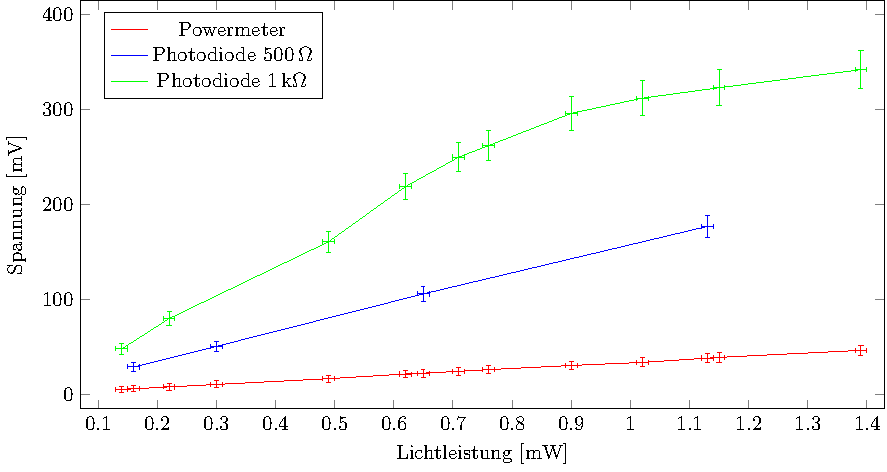
\includegraphics[width=1\linewidth]{graphs/fotodiode/diode.pdf}
	\caption[Vermessung einer Photodiode]{
		Spannungen gemessen über je einen zu einer Photodiode parallel geschalteten Widerstand mit 500 und \unit[1000]{$\Omega$}. Zusätzlich ist der Verlauf der Spannung eines Powermeters aufgetragen.
	}
	\label{fig:photodiode}
\end{figure}

Daher wurde der Aufbau mit kleineren Widerstandswerten von 500 und \unit[1000]{$\Omega$} getestet. Die gemessenen Spannungen sowie die dazu vom Powermeter abgelesenen Werte für die Lichtleistung sind in Abbildung~\ref{fig:photodiode} aufgetragen.

Es ist für \unit[1]{$k\Omega$} eine Sättigung ab etwa \unit[0,9]{mW} erkennbar, die Variante mit \unit[500]{$\Omega$} weist im gesamten Messbereich ein lineares Verhalten auf. Die Fehlerbalken in der x-Achse wurden zu \unit[0,01]{mW} gewählt, da das verwendete Powermeter nur zwei Nachkommastellen anzeigte. Der Fehler in der y-Achse wurde auf etwa 5\% gewählt.

%Bei dieser Wellenlänge hat die Photodiode eine Effizienz von etwa \unit[20]{\%} bei der Umwandlung von Licht zu Strom. Bei \unit[660]{nm} (Frequenz des Lasers) etwa \unit[40]{\%}.

\subsubsection*{Auswertung}

Um aus dem Spannungsabfall über den zu der Photodiode parallel geschalteten Widerstand eine Lichtleistung bestimmen zu können ist ein lineares Verhalten von Vorteil. So kann direkt aus der Spannung mittels eines Faktors die Leistung berechnet werden. Mit einem Widerstand von $\unit[1]{k\Omega}$ ist ein lineares Verhalten nur im Bereich bis etwa \unit[0,7]{mW} zu beobachten. Darüber hinaus sättigt die Spannung. Vermutlich ließe sich mit einer Wertetabelle (erstellt mit Hilfe des kommerziellen Powermeters) auch weit über diesen Bereich hinaus sinnvoll die Lichtleistung berechnen.

Für den $\unit[500]{\Omega}$ Widerstand ist bis zur maximal vermessenen Lichtleistung $P_L$ von etwa \unit[1,1]{mW} keine Sättigung festzustellen (vgl. Abb.~\ref{fig:photodiode}). Für den vorgesehen Verwendungszweck empfiehlt sich daher die Verwendung eines Widerstandswertes in der Nähe von $\unit[500]{\Omega}$. Mit Hilfe der Software \textit{QtiPlot} wurde eine Lineare Regression mit der Formel $U=a\cdot P_L + b$ über die aufgenommenen Datenpunkte ausgeführt. Daraus ergeben sich die Werte $b=(5,2346 \pm 1,1515) \unit{mW} $ und $a= 152,6614\pm 1,7095) \unitfrac{W}{V}$. Die Standardabweichung liegt bei $1,28$.\\


Das beobachtet Verhalten lässt sich sehr gut erklären, indem man einen PN-Übergang in der Photodiode mit einer Bandlücke von etwa \unit[500]{mV} annimmt. Für eine feste Frequenz kann die Lichtleistung direkt in die Anzahl der Photonen $N_{Ph}$ umgerechnet werden: $N_{Ph} = \nicefrac{P_L}{E_{Ph}}$, wobei $E_{Ph}=\hbar \omega_{Ph}$ die Energie pro Photon ist. Jedes dieser Photonen treibt mit einer Wahrscheinlichkeit, entsprechend der Quanteneffizienz des Überganges für die Frequenz der Photonen $\omega_{Ph}$, genau einen elektronischen Übergang. So führt eine bestimmt Leistung zu einer bestimmten Anzahl angeregter Elektronen. Dies entspricht bei kompletter Besetzungsinversion der Zustände einem konstantem Strom und somit Spannungsabfall über den Widerstand. Sobald dieser Widerstand jedoch so groß gewählt wird, dass der Spannungsabfall in etwa dem Bandlückenpotential entspricht, wird die Besetzungsinversion aufgehoben. Dadurch sinkt die Quanteneffizienz und folglich der Stromfluss. Folglich sinkt die abgefallene Spannung über den Widerstand. Dies erklärt das lineare Verhalten bei kleinen Widerständen beziehungsweise Lichtleistungen und das Sättigungsverhalten ab etwa \unit[250]{mV}.

	\subsection{4f-Aufbau}
	% !TeX root = ../praktikum.tex
% !TeX encoding = UTF-8
% !Tex spellcheck = de_DE

Im letzten Versuchsteil wurde der Laserstrahl am anderen Ende der Glasfaser ausgekoppelt und auf einen optischen Pfad gesandt, um Abbildungen von Objekten und deren Fourierspektren, sowie die Veränderung der Abbildung bei Maniplation des Fourierspektrums zu beobachten. Hierfür wurde hinter dem Faserauskoppler der Aufbau aus Abbildung \ref{fig:4f-aufbau} realisiert.

\begin{figure}[h]
	\centering
	\includegraphics[width=1\linewidth]{graphs/versuchsaufbau/4f-aufbau.pdf}
	\caption[Schematische Skizze des 4f-Aufbaus]{
		Schematische Skizze des 4f-Aufbaus. Der Laserstrahl passiert nach Verlassen des Auskopplers eine $\nicefrac{\lambda}{2}$-Platte und anschließend einen Strahlteiler. Der zweite Teil des Strahls, welcher vom Strahlteiler abgelenkt wird, trifft auf eine Strahlblockierung und wird nicht weiter verwendet. Zwischen Linse 2 und 3 befindet sich die Halterung für das Objekt/Dia, in der Fourierebene wird entweder eine zweite Kamera oder ein Filter positioniert. Die CCD Kamera am Ende des Strahlengangs befindet sich in der Abbildungsebene des Aufbaus.
	}
	\label{fig:4f-aufbau}
\end{figure}

In diesem, sogenannten 4f-Aufbau, passierte der Laserstrahl nach der Reflektion am ersten Spiegel eine $\nicefrac{\lambda}{2}$-Platte und dahinter einen Strahlteiler. Mithilfe des Strahlteilers wurde eine eindeutige Polarisierung sicher gestellt, während mit dem Plättchen die Lichtmenge der durchlässigen Polarisation eingestellt werden konnte.\\

Um die abzubildenden Objekte vollständig ausleuchten zu können, wurde der Laserstrahl in diesem Aufbau mit Hilfe der ersten beiden Linsen aufgeweitet und wieder kollimiert. Im Brennpunkt der dritten Linse befand sich ein Objektträger in der Gegenstandsebene. In diesem wurden die abzubildenden Objekte angebracht. Die Fourierebene befindet sich im Brennpunkt der Linsen 3 und 4. Nach der vierten Linse wird der Strahl erneut kollimiert und trifft auf die CCD Kamera, Kamera 1. Hier wird das Objekt möglichst originalgetreu abgebildet. Um Aufnahmen der Fourierspektren zu erhalten, wurde bei Bedarf eine zweite Kamera, Kamera 2, in der Fourierebene montiert. \\ 

Verwendet wurden hierbei Linsen der Brennweiten wie folgt: Linse 1 mit $f_{1}=\unit[20]{mm}$, Linse 2 mit $f_{2}=\unit[200]{mm}$, Linse 3 und 4 mit $f_{3}=f_{4}=\unit[100]{mm}$. Direkt hinter der Auskopplung wurde zusätzlich ein Spiegel, optimiert für Wellenlängen zwischen \unit[400-700]{nm}, in den 4f-Aufbau aufgenommen, um den Verlauf des Laserstrahls im optischen Pfad besser feinjustieren zu können. Leider wurde die Strahlqualität durch diesen stark beeinträchtigt, so dass zusätzlich ein Pinhole zwischen Linse 1 und 2 notwendig war, um eine gaußähnliche Strahlmode zu erhalten.\\


\begin{figure}[h]
	\centering
	\includegraphics[width=0.7\linewidth]{images/4f-anfang.JPG}
	\caption[Vorderer Teil des 4f-Aufbaus]{
		Vorderer Teil des realisierten 4f-Aufbaus. Am rechten Bildrand ist das Pinhole hinter Linse 1 zu sehen.
	}
	\label{fig:_DSC7961}
\end{figure}

\begin{figure}[ht]
	\centering
	\includegraphicsRS[width=0.43\linewidth]{images/_DSC7988.JPG}~
	\includegraphicsRS[width=0.43\linewidth]{images/IMG_2223.jpg}
	%\vspace{2cm}\hspace{2cm}
	\caption{
		\textbf{Links:} Mode des Laserstrahls am Ende des optischen Pfades vor Einbau des Pinholes.\\
		\textbf{Rechts:} Mode des Laserstrahls am Ende des optischen Pfades nach Einbau des Pinholes.
	}
	\label{fig:_DSC7988}
\end{figure}


Als Hilfsmittel bei der Justage des 4f-Aufbaus wurde hier eine Iris verwendet. Mit dieser konnte beispielsweise die Kollimierung des Laserstrahls hinter Linse 2 Überprüft werden, indem die Öffnung der Iris auf die Strahlbreite eingestellt wurde und anschließenend entlang des optischen Pfades verschoben wurde. Die Justage der Linse konnte somit verbessert werden. Außerdem ließ sich mit Hilfe der Iris über die gleiche Vorgehensweise die Höhe des Strahls kontrollieren und diese dann anhand der Technik des Walkens optimieren. 


\begin{comment}
\begin{figure}
	\centering
	\includegraphicsRS[width=0.7\linewidth, angle=90]{images/_DSC7967.JPG}
	\caption{Foto des hier realisierten 4f-Aufbaus.}
	\label{fig:_DSC7967}
\end{figure}
\end{comment}

\clearpage



	\label{chap:abb+ft}
		
		
	\section{Experimentelle Durchführung und Auswertung}
	\label{chap:auswertung}
	In diesem Teil sollen Bildinformationen eines Objektes fouriertransformiert, die Transformierte aufgenommen, mit Hilfe verschiedener Filter manipuliert und anschließend rücktransformiert werden. Hierfür werden Objekte, wie z.B. Dias in die Objektebene eingebracht. In der Fourierebene können  Filter oder eine Kamera montiert werden, um die Fouriertransformierte manipulieren oder aufnehmen zu können. Eine Kamera dient zur Aufnahme der Rücktransformierten.\\
	
	Die fünf verwendeten Objektdias werden als \textit{Objekte 1 bis 5} (siehe Abbildung~\ref{fig:Objekte-aus-Anleitungsheft}) bezeichnet. Objekt 1-4 enthalten mehrere Motive, die einzeln untersucht werden.
	
	\begin{figure}[h]
		\centering
		\includegraphicsRS[width=0.15\textwidth][.15]{images/Anleitungsheft/objekt1.png}~~
		\includegraphicsRS[width=0.15\textwidth][.15]{images/Anleitungsheft/objekt2.png}~~
		\includegraphicsRS[width=0.15\textwidth][.15]{images/Anleitungsheft/objekt3.png}~~
		\includegraphicsRS[width=0.15\textwidth][.15]{images/Anleitungsheft/objekt4.png}~~
		\includegraphicsRS[width=0.15\textwidth][.15]{images/Anleitungsheft/objekt5.png}
		\caption[Die zur Messung verwendeten Diamotive]{
			Darstellung der zur Messung verwendeten Dias. Im Text werden diese Objektdias mit Objekt 1 bis 5, von links nach rechts, bezeichnet.
		}
		\label{fig:Objekte-aus-Anleitungsheft}
	\end{figure}
	
	Anhand der Dias wurden zunächst sowohl Kamera 1, als auch Kamera 2 nachjustiert, bis ein möglichst scharfes Bild auf dem über das Programm \textit{uc480 Viewer-DCC1545M-ID} angeschlossenen Bildschirm zu erkennen war. %In den nachfolgenden Teilen werden für die Objekte Aufnahmen in der Abbildungsebene und zugehörig zu jeder Einstellung auch in der Fourierebene gemacht. Zudem werden für die Objekte 4 und 5 verschiedene Filter in die Fourierebene gestellt und Aufnahmen der Kamera 1 in der Abbildungsebene gemacht und untersucht. Für Objekt 4 wurde hierzu ein Tiefpass und mehrere Breitbandfilter verwendet. Für Objekt 5 wurde ein Halbebenenfilter horizontal, vertikal und diagonal in die Fourierebene gehalten.\\
		
	% !TeX root = ../praktikum.tex
% !TeX encoding = UTF-8
% !Tex spellcheck = de_DE



\subsection{Untersuchungen an Gittern}
In diesem Abschnitt werden verschiedene Gitter des Objektes 3 untersucht. Dazu wurde das entsprechende Dia in der Objektebene montiert. Das gewünschte Motiv auf der Schablone wurde möglichst mittig in dem Strahl montiert. Mit einer Papierschablone wurde verhindert, das Motive beleuchtet werden, die gerade nicht untersucht wurden, da dies eine Überlagerung mehrerer Fourierspektren zur Folge hätte (vgl. Abb.~\ref{fig:kreuzgitter_und_spektrum}~a und b) und das Untersuchen eines einzelnen Spektrums unmöglich machen würde. Für jedes der neun Motive wurde je ein Bild in der Fourierebene sowie in der Abbildungsebene aufgenommen. Bei dem Einschieben der Objekte lässt sich feststellen, dass die Bewegungsrichtung der Abbildung entgegengesetzt zu der des echten Motives ist. Ebenso sieht man bei asymmetrischen Objekten, dass diese "auf dem Kopf stehen".


\begin{figure}[ht]
	\centering
	%\includegraphicsRS[width=0.6\textwidth]{images/Regina/abb13.jpg}
	\includegraphics{images/Regina/abb13.pdf}
	\caption[Gitter mit Fourierspektrum]{
		Vertikales Gitter (a) und das dazugehörige Beugungsbild (b), welches das Fourierspektrum darstellt. Das Fourierspektrum weist erneut Beugungsbilder als eine Unterstruktur auf (c).
	}
	\label{fig:gitter_und_spektrum}
\end{figure}

Für eines der Gittermotive aus der ersten Reihe sind diese Aufnahmen in Abbildung~\ref{fig:gitter_und_spektrum} abgebildet. In der Fourierebene ist eine Reihe von Punkten zu sehen. Die Motive der zweiten Reihe ergeben in beiden Ebenen jeweils das gleiche Bild, jedoch um $90^\circ$ gedreht. Je dichter die Gitterlinien beieinander liegen, desto weiter liegen die Punkte in der Fourierebene auseinander.

Die Abbildung eines Motiv der letzten Reihe (Kreuzgitter) ist in Abbildung~\ref{fig:kreuzgitter_und_spektrum}~a abgebildet, b zeigt das Bild in der Fourierebene (\textit{Fourierspektrum}). Zusätzlich zeigt die Abbildung~\ref{fig:kreuzgitter_und_spektrum}c das Fourierspektrum, wenn mehrere Motive gleichzeitig beleuchtet werden. Die Kreuzgitter erzeugen in der Fourierebene zwei senkrechte Punktreihen, wobei der Punktabstand mit zunehmenden Gitterlinienabstand abnimmt.

\begin{figure}[ht]
	\centering
	%\includegraphicsRS[width=0.4\textwidth]{images/Regina/abb14.jpg}
	\includegraphics{images/Regina/abb14.pdf}
	\caption[Kreuzgitter mit Fourierspektrum]{
		Kreuzgitter (a) und das dazugehörige Beugungsbild (b), das das Fourierspektrum darstellt. Eine Überlagerung von mehreren Fourierspektren (c).
	}
	\label{fig:kreuzgitter_und_spektrum}
\end{figure}



\subsubsection*{Auswertung}
Das Zustandekommen und Aussehen einer Abbildung kann durch die aus der zweifachen 
Da das Licht im vertikalen Gitter nur in der vertikalen Richtung gebeugt wird, bilden sich die Intensitätsschwankungen in der Fourierebene ausschließlich in horizontaler Richtung aus. Somit wurde dort eine senkrecht zu dem Gitter stehende Reihe aus Interferenzmaxi- und -minima beobachtet: Vergleich Abbildung~\ref{fig:gitter_und_spektrum}. Das Drehen des Motives sorgt ebenfalls für ein gedrehtes Bild in der Fourierebene. Dies ist direkt aus der Beugungstheorie an Gittern ersichtlich. Die Änderungen des Spektrums unter Variation des Spaltabstandes zu beobachten waren, lassen sich mit der mathematischen Eigenschaft der Ähnlichkeit der FT erklären (s. Abschnitt~\ref{chap:math_basic}), allerdings folgt auch dies direkt aus der Beugungstheorie an Gittern beziehungsweise Mehrfachspalten.\\

Bei einem Kreuzgitter findet die Beugung in horizontaler und vertikaler Richtung statt, welches einer Kreuzform in der Fourierebene entspricht. Das Motiv entspricht also einer Überlagerung zweier um $90^\circ$ gedrehten Gitter. Nach der mathematischen Eigenschaft der Linearität der FT (s. Abschnitt~\ref{chap:math_basic}) folgt somit auch die Überlagerung der entsprechenden Spektren. Dies war sehr gut zu beobachten.

Wenn mehrere Motive beleuchtet wurden ergab sich in der Fourierebene die in Abbildung~\ref{fig:kreuzgitter_und_spektrum}~c dargestellt kreuzförmige Anordnung. Diese zeigt nicht ein einzelnes Kreuz, sondern mehrere Kreuze mit einem bestimmten Abstand voneinander. Das Auftreten mehrerer Kreuze lässt sich analog mit der Linearitätseigenschaft der FT erklären. 


Da wir in der Objektebene ein Dia als Quelle unserer Abbildungen verwendet haben und dieses Dia wie in Abb. 8 %TODO REF!!!
 dargestellt (Objekt 3) in der untersten Reihe drei verschiedene Kreuzgitter und darüber weitere horizontale und vertikale Gitter aufwies, wurden diese ebenfalls angestrahlt und lieferten die zusätzlichen Kreuze. Um diese zu unterbinden, wurden die anderen Objekte, auch bei den nachfolgenden verwendeten Objekten, mit schwarzen Klebeband überklebt. Durch diese Modifizierung der Dias konnte das erwartete einzige Kreuz erzeugt werden (Abb.~\ref{fig:gitter_und_spektrum}~b).

Sowohl bei dem vertikalen Gitter als auch bei dem Kreuzgitter ist in der Fourierebene im Zentrum der Beugungsbilder eine maximale Intensität zu erkennen. Dieses Maximum entsteht durch das Kreuzen der mittleren horizontalen oder im Kreuzgitter der vertikalen und
horizontalen Beugungsbilder. Dabei ist bei jedem weiteren Kreuzpunkt erneut eine erhöhte Intensität zu erkennen, die aber nach außen hin abnimmt. Diese lässt sich ebenfalls bei einem
Doppelspalt beobachten, wobei das Intensitätsmaximum nullter Ordnung am stärksten ist und die Maxima höherer Ordnungen immer schwächer werden ($\nicefrac{sin(x)}{x}$). Dabei nimmt die Intensität im Zentrum mit zunehmen kleiner werdenden Gitterkonstante zu.
Weiterhin wiesen alle Intensitätsmaxima eine Unterstruktur auf. Diese Unterstrukturen entstehen durch die Interferenz der Haupt- und Nebenmaxima aller Spalte des Gitters. Somit entsteht im Gegensatz zu einem Doppelspalt das Beugungsbild eines Gitter aus Vielfachinterferenzen. Diese Eigenschaft entspricht der mathematischen geforderten Linearität. Denn das Beugungsbild eines Gitters kann somit durch das aufsummieren der einzelnen Beugungsbilder des Einzelspaltes erzeugt werden (siehe 1.1. Linearität%TODO:REF!!!
).


\subsection{Erzeugung von Beugungsbilder von Punkten}
\subsubsection*{Auswertung}

Bei der optische Fouriertransformation gilt für Punkte wie bereits für Gittern erläutert die Linearität, so dass das erzeugte Beugungsbild in der Fourierebene sich aus der Summe der Beugungsbilder der einzelnen Punkte ergibt. Das Beugungsbild eines Punktes besteht aus konzentrischen Ringen, dessen Breite und Intensität nach außen abnehmen. Durch das Verschiebungtheorem der Fouriertransformation ist gegeben, dass sich das Beugungsbild der beiden Punkte an einer Position befinden, trotz der unterschiedlichen Position der Punkte. Bei zwei Punkten ergibt sich somit erneut eine Vielfachinterferenz analog zum Gitter, welches erneut durch Unterstrukturen in den konzentrischen Ringen erkennbar wird (Abb.~\ref{fig:punktpaare_verschieden_und_spektren}~b, d). Mit zunehmenden Abstand zwischen den Punkten werden die Unterstrukturen feiner. Dieses entspricht dem Ähnlichkeitstheorem (siehe 1.1. Ähnlichkeit%TODO:REF!!!
), so dass mit zunehmenden Abständen der Punkte sich die Beugungsmaxima annähern, bzw. die Abstände zwischen diesen kleiner werden. Für ein Gitter bedeutet dieses, je größer die Gitterkonstante ist, d.h. je größer der Abstand zwischen den Spalten ist, desto kleiner wird der Abstand zwischen den einzelnen Maxima und Minima.

\begin{figure}[h]
	\centering
	%\includegraphicsRS[width=0.3\textwidth]{images/Regina/abb15.jpg}
	\includegraphics{images/Regina/abb15.pdf}
	\caption[Punktpaare unterschiedlicher Abstände und Fourierspektren]{
		Punktpaare mit unterschiedlichen Abständen zueinander (a1, b1) und die dazugehörigen Beugungsbilder in der Fourierebene (a2, b2).
	}
	\label{fig:punktpaare_verschieden_und_spektren}
\end{figure}


\begin{figure}[h]
	\centering
	%\includegraphicsRS[width=0.3\linewidth]{images/Regina/abb16.jpg}
	\includegraphics{images/Regina/abb16.pdf}
	\caption[Punktpaare gleicher Abstände und Fourierspektren]{
		Punktpaare mit gleichen Abständen und unterschiedlicher Größe (a1, b1, c1) und die dazugehörigen Beugungsbilder in der Fourierebene (a2, b2, c2).
	}
	\label{fig:punktpaare_gleich_und_spektren}
\end{figure}

Bei den geringsten Abstand sind im Beugungsbild neben den konzentrischen Formen auch vertikale Gitter zu erkennen (Abb.~\ref{fig:punktpaare_verschieden_und_spektren}~b2). Diese Gitterform stellen die bereits erwähnten Unterstrukturen der Beugungsbilder dar. Zwei Punkte ergeben in der Fourierebene als
Unterstruktur eine Linienstruktur senkrecht zur Verbindungslinie der beiden Punkte. Diese ergeben sich somit ebenfalls bei zwei Punkten mit höheren Abstand, sind aber wegen des kleinen Abstand zwischen den Spalten des vertikalen Gitters in der Fourierebene schlecht zu erkennen, da sich die Fouriertransformierte reziprok verhält (Ähnlichkeitstheorem). Bei kleinere Abstand zwischen den Punkten, vergrößert sich der Abstand der Spalten im vertikalen Gitter, und ist dadurch erkennbar. Diese Unterstrukturen sind noch ausgeprägter bei gleichbleibenden Abstand und kleinerer Größe der Punkte zu erkennen (Abb.~\ref{fig:punktpaare_gleich_und_spektren}~b2, c2). Die Intensitätsmaxima sind bei den kleineren Punkte durch ihren größeren Abstand zueinander kleiner ausgeprägt als bei den größeren Punkten. Somit weist das Hauptmotiv des Beugungsbild eine geringe Intensität auf, wodurch die Unterstruktur einfacher zu erkennen
ist.
Auch bei dem Beugungsbild eines Punktringes (Abb.~\ref{fig:punktringe_und_spektrum}) sind Unterstrukturen in der Fourierebene zu erkennen, die sich durch die Anordnung der acht Punkte ergeben. Zwei Punkte weisen eine senkrechte Linienstruktur zur Verbindungslinie auf, so dass sich bei acht Punkten vier Linienstrukturen (horizontal, vertikal, beide Diagonale) ergeben. Wenn sich diese Strukturen kreuzen, ergeben sich acht Schnittpunkte und somit eine Unterstrukturen, die wie Achtecke aussehen (Abb.~\ref{fig:punktringe_ausschnitt}).

\begin{figure}[h]
	\centering
	%\includegraphicsRS[width=0.10\linewidth]{images/Regina/abb17.jpg}
	\includegraphics{images/Regina/abb17.pdf}
	\caption[Punktringe mit Fourierspektren]{
		Punktringe (a1) und Punktringe mit zusätzlichem Punkt in unterschiedlicher Größe (b1, c1) und die dazugehörigen Beugungsbilder in der Fourierebene (a2-c2).
	}
	\label{fig:punktringe_und_spektrum}
\end{figure}

\begin{figure}[h]
	\centering
	\includegraphicsRS[width=0.42\textwidth]{images/Regina/abb18.jpg}
	\caption[Beugungsbild der Punktringe mit vergrößertem Ausschnitt]{
		Ausschnitt aus dem Beugungsbild des Punktringes, welche die Unterstruktur eines Achtecks zeigt.
	}
	\label{fig:punktringe_ausschnitt}
\end{figure}

Bei einem Punktkreis mit einem zusätzlichen Punkt ist das Beugungsbild nicht mehr symmetrisch und die Asymmetrie nimmt mit größer werdenden Punkt zu (Abb.~\ref{fig:punktpaare_gleich_und_spektren}~b, c).


\subsection{Erzeugung von Beugungsbilder von Buchstaben und Zahlen}
\subsubsection*{Auswertung}

Der Buchstabe D besteht aus sowohl horizontalen, vertikalen Linien und runden Elementen (Abb.~\ref{fig:ziffern_mit_spektren}~a1). Das Beugungsbild ergibt sich somit aus der Summe der Beugungsbilder dieser verschiedenen Formen. Die horizontalen Linien bilden ein Fourierspektrum in der Horizontalen und die vertikalen Linien in der Vertikalen mit den jeweiligen Maxima und Minima und Unterstrukturen (Abb.~\ref{fig:ziffern_mit_spektren}~a2). Die runde Form erzeugt in dem Beugungsbild konzentrische Ringe mit abnehmender Intensität, entsprechend dem Beugungsbild von Punkten. Da der Buchstabe D durch horizontale und vertikalen Linien dominiert wird, ist auch das Beugungsbild stark davon geprägt, so dass die konzentrischen Ringe durch eine geringere Intensität auch schlechter zu erkennen sind.

\begin{figure}[h]
	\centering
	%\includegraphicsRS[width=0.4\textwidth]{images/Regina/abb19.jpg}
	\includegraphics{images/Regina/abb19.pdf}
	\caption[Ziffern mit Fourierspektren]{
		Buchstabe D (a1) und Zahl 4 (b1) und die dazugehörigen Beugungsbilder in der Fourierebene (a2 und b2).
	}
	\label{fig:ziffern_mit_spektren}
\end{figure}

Die Zahl 4 besteht lediglich aus Linien, wobei neben horizontalen und vertikalen Linien ebenfalls diagonale Linien vorhanden sind (Abb.~\ref{fig:ziffern_mit_spektren}~b1). Da das erzeugten Beugungsbild eines Gitters eine senkrecht auf dem Gitter stehende Punktereiche aus Interferenzmaxima und –minima darstellt, ist zusätzlich zu der horizontalen und vertikalen Richtung ein Fourierspektrum in der Diagonalen senkrecht zur der Diagonale der Objektebene anzufinden (Abb.~\ref{fig:ziffern_mit_spektren}~b2).

\subsection{Erzeugung von Beugungsbildern des Fourierhauses}
\subsubsection*{Auswertung}

Das Fourierhaus ist ein Haus, welches aus Gittern mit gleichen Gitterkonstanten und unterschiedlicher Ausrichtungen der Gitter besteht (Abb.~\ref{fig:fourierhaus_mit_filtern}~a1). Die verschiedenen Gitter entsprechen verschiedenen Bauelementen im Haus. Die Wand besteht aus einem vertikalen Gitter, das Dach aus einem horizontalen Gitter und die Tür und der Schornstein werden aus diagonalen Gittern in entgegen gerichteten Richtung erstellt. Die Fouriertransformation dieses Fourierhauses ergibt das in Abbildung~\ref{fig:fourierhaus_mit_filtern}a2 dargestellte Beugungsbild. Die vier verschiedenen Orientierung der Gitter sind in der Fourierebene ebenfalls durch vier verschiedene Orientierungen dargestellt, die jeweils senkrecht auf der Objektebene stehen. Da die Gitterkonstante des Fourierhauses im Vergleich zu den in Abbildung~\ref{fig:gitter_und_spektrum} und \ref{fig:kreuzgitter_und_spektrum} gezeigten Gittern sehr viel kleiner ist, sind die Abstände zwischen den Maxima im Fourierspektrum deutlich größer (siehe 1.1. Ähnlichkeit%TODO REF!!!
 ) und die Intensität im Zentrum erhöht.


\subsection{Optische Filterung des Fourierhauses durch eine Schneide}
\subsubsection*{Auswertung}

Für eine optische Filterung wurden verschiedene Filter in der Fourierebene des 4f-Aufbaus eingesetzt (siehe Abb.4%TODO:REF!!!
). Zuerst wurde das Fourierhaus durch Filter manipuliert. Durch die Verwendung einer Schneide, die bestimmte Frequenzbereiche durch das Abdecken der Frequenzspektren durch lichtundurchlässigen Material herausfiltert, konnten verschieden Bauelemente jeweils heraus gefiltert werden. Durch zwei Schneiden wurden in dem Fourierebene das Beugungsbild so abgedeckt, dass lediglich das vertikale Fourierspektrum des Daches und das diagonale Fourierspektrum der Tür übrig blieben (Abb.~\ref{fig:fourierhaus_und_spektrum}~b1). Somit waren in der Abbildungsebene nur die näherungsweise horizontalen Linien des Daches und der Tür sichtbar (Abb.~\ref{fig:fourierhaus_und_spektrum}~b2). Analog wurden durch das Abdecken mit dem Filter erreicht, dass nur das horizontale Fourierspektrum sichtbar war und somit nur vertikale Linien (Wand) in der Abbildungsebene sichtbar wurden (Abb.~\ref{fig:fourierhaus_und_spektrum}~c1, c2). Als letztes wurde, durch das Blockieren des diagonalen Fourierspektrums, lediglich der Schonstein ausgeblendet (Abb.~\ref{fig:fourierhaus_und_spektrum}~d1, d2).

\begin{figure}[h]
	\centering
	%\includegraphicsRS[width=0.75\textwidth]{images/Regina/abb21.jpg}
	\includegraphics[scale=1]{images/Regina/abb21.pdf}
	
	\caption[Fourierhaus mit verschiedenen Filtern]{
		Durch zwei Schneiden (blau schraffiert) werden verschiedene Teile der Fourierspektren in der Fourierebene herausgefiltert (oben), welches in der Abbildungsebene zum Verschwinden einzelner Teile führt (unten).
	}
	\label{fig:fourierhaus_mit_filtern}
\end{figure}

\subsection{Optische Filterung durch Hochpass-, Tiefpass- und Breitbandfilter}

Als Nächstes wurde die Abbildung eines Fingerabdrucks auf einem Glasplättchen zunächst ohne Filter aufgenommen. Hierbei war in der Abbildungsebene relativ wenig zu erkennen (siehe Abbildung \ref{fig:example20_Hochpass}~a). Anschließend wurde die Abbildung mit einem in der Fourierebene befindlichen Hochpass- und einem Halbebenenfilter aufgenommen. Zudem wird mit Kamera 2 das Fourierspektrum des Fingerabdrucks photographiert. Zu beobachten war hier, dass die Konturen des Fingerabdrucks in der Abbildung mit Hilfe der Filter deutlich besser erkennbar gemacht werden konnten (vgl Abbildung \ref{fig:example20_Hochpass}~b, c).\\


\begin{figure}[h]
	\centering
	%\includegraphicsRS[width=0.6\linewidth]{images/example20_Hochpass.png}\\
	%\includegraphicsRS[width=0.6\linewidth]{images/example21_Halbebenenfilter.png}
	\includegraphics{images/ergebniss_Fingerab/abb.pdf}
	%TODO: Nur eines dieser Bilder!
	\caption{
		Der Fettabdruck eines Fingers in der Abbildungsebene ohne Filter (a) und mit Hochpassfiltern (b, c).
	}
	\label{fig:example20_Hochpass}
\end{figure}

\subsubsection*{Auswertung}

Als Erstes wird ein Breitbandfilter bei der Zahl vier eingesetzt. Da der Breitbandfilter sowohl kleinere und größere Frequenzen herausfiltert und somit nur eine bestimmtes Frequenzintervall durchlässt, werden die Flächen unterdrückt und Ränder als Doppellinien dargestellt. Beim Breitbandfilter C (Abb %TODO REF!!!
c) konnte dieser Effekt am besten beobachtet werden (Abb.~\ref{fig:vier_mit_breitband}~b). Bei den Breitbandfilter B und A ist die Filterwirkung so stark, dass nur
ein sehr kleiner Frequenzintervall durchgelassen wird und dadurch die Zahl vier kaum noch zu erkennen ist (Abb. \ref{fig:vier_mit_breitband}c, d).

\begin{figure}[h]
	\centering
	%\includegraphicsRS[width=0.4\textwidth]{images/Regina/abb22.jpg}
	\includegraphics{images/Regina/abb22.pdf}
	\caption[Zahl 4 mit Breitbandfiltern]{
		Die Zahl vier in  der Abbildungsebene ohne Filter (a) und mit dem Breitbandfilter C (b), B (c) und A (d) gefilterte Bilder der Zahl vier.
	}
	\label{fig:vier_mit_breitband}
\end{figure}

Durch die Verwendung eines Tiefpassfilters wurden die niedrigen Frequenzen durchgelassen und somit die hohen Frequenzen herausgefiltert. Diese bewirken eine niedrigere Auflösung des
Bildes, da die Flächen unterdrückt werden, welches in der Abbildung~\ref{fig:vier_mit_breitband}~b dargestellt ist bei der Zahl 4 und dem Buchstaben D dargestellt ist. Da diese beiden Objekte keine innere Flächenstrukturen wie Gitter aufweisen, ist dieser Effekt nicht zu erkennen.
Im Gegenteil dazu wurden bei einem Fingerabdruck ein Hochpassfilter eingesetzt, der die niedrigen Frequenzen herausgefiltert, welches zu einer Hervorhebung der Kanten führte (Abb.~\ref{fig:vier_mit_tiefpass}~b). In der Bildverarbeitung werden die Tiefpass- (Weichzeichner) und Hochpassfilter (Kantenerkennung) häufig verwendet.

\begin{figure}[h]
	\centering
	%\includegraphicsRS[width=0.4\textwidth]{images/Regina/abb23.jpg}
	\includegraphics{images/Regina/abb23.pdf}
	\caption[Zahl 4 mit Tiefpassfilter]{
		Die Zahl vier in der Abbildungsebene (a) und mit dem Tiefpassfilter (b) gefilterte Abbildung der Zahl vier.
	}
	\label{fig:vier_mit_tiefpass}
\end{figure}


\begin{figure}[h]
	\centering
	\includegraphics{images/ergebniss_D/abb.pdf}
	\caption{
		Der Buchstabe D des Objekts 4 in der Abbildungsebene ohne Filter (a), mit dem Filter 1D (b), 1C (c), 1B (d).
	}
	\label{fig:example10_Filter1B}
\end{figure}


\subsection{Schlierenverfahren durch Verwendung eines Halbebenenfilters}

Als Letztes wurde ein Teelicht auf die Position des Objektträgers gestellt und ein Halbebenenfilter in der Fourierebene installiert. Mit Kamera 1 wurden mehrere Abbildungen aufgenommen, um die Strömungsbewegungen oberhalb der Flamme beobachten zu können. Zum Vergleich wurde zudem eine Aufnahme mit Halbebenenfilter, jedoch ohne Teelicht gemacht (siehe Abb.~\ref{fig:Halbebenenfilter_mit_und_ohne_Teelicht}). Auf dieser Beispielaufnahme sind deutliche Verzerrungen des Lichts aufgrund der Luftströmungen über der Flamme des Teelichts zu erkennen. 

\begin{figure}[h]
	\centering
	%\includegraphicsRS[width=0.7\linewidth]{images/example22_Halbebenenfilter_mit_und_ohne_Teelicht.png}
	\includegraphics{images/ergebniss_Teelicht/abb.pdf}
	\caption[Schlieren]{
		Aufnahme ohne Objekt in der Abbildungsebene mit Halbebenenfilter ohne Teelicht (a) und mit Teelicht (b, c).
	}
	\label{fig:Halbebenenfilter_mit_und_ohne_Teelicht}
\end{figure}


\subsubsection*{Auswertung}

Mit Hilfe eines Halbebenenfilters (Schneide) wurden die durch   eine brennende Kerze erzeugten Schlieren dargestellt (Abb.~\ref{fig:Halbebenenfilter_mit_und_ohne_Teelicht}). Als Schlieren werden Bereiche bezeichnet, die sich von ihrer Umgebung  in  der  Dichte  bzw.  im  Brechungsindex  unterscheiden,  welche  in  unseren Versuch die durch  die  Kerze erzeugten Luftströmungen darstellten. Bei diesem Versuchsaufbau  wurde  das  Prinzip  genutzt,  dass  parallele  Strahlenbündel  beim  Durchgang durch   ein   inhomogenes Dichtefeld   unterschiedlich   stark   abgelenkt   werden.   Durch   die eingesetzte  Schneide,  wurden  die  Anteile  des  gebrochenen  Lichts  ausgeblendet,  so  dass richtungsabhängige  Brechzahl-  bzw.  Dichtegradienten auf  dem  Projektionsschirm  sichtbar wurden. Dabei ist die Intensitätsverteilung im   Bild   proportional   zum   Quadrat   der Phasenverschiebung   durch   das   Objekt.   Somit   ermöglicht es dieses Verfahren, eine Phasenverschiebung sichtbar zu machen. 

	
	\clearpage
	\newpage
	
	\section{Fazit} %Diskussion der physikalischen Ergebnisse
	% !TeX root = ../praktikum.tex
% !TeX encoding = UTF-8
% !Tex spellcheck = de_DE



Durch diesen Versuch werden die theoretischen mathematischen Grundlagen der Fouriertransformation anhand anschaulicher Experimente nachvollziehbar. Dabei ist der Vergleich der Eigenschaften der Linse und dem entsprechenden Aufbau mit den geforderten. Eigenschaften einer Funktion (Linearität, Ähnlichkeit, Verschiebung, Faltung) für eine Fouriertransformation für das Verständnis sehr nützlich. Insbesondere wird dies durch die Verwendung von verschiedenen Filtern und die daraus folgende Manipulation der Bilder vermittelt. 

Der selbständige Aufbau, der die Optimierung des Diodenlasers als auch des Strahlengangs umfasste, veranschaulichte deutlich die Herausforderungen des Versuchs und somit die Herausforderungen beim Experimentieren und somit de
m Umgang mit der Ausrüstung in der Optomechanik. Dabei ist viel Geduld, z.B. bei der Einkopplung erforderlich, sowie auch Kreativität, was uns anhand des Baus der Photodiodezur Messung der Effizienz des Lasers verdeutlicht wurde. Weiterhin zeigte das Justieren des Strahlengangs, dass bereits kleinste Veränderungen einen enormen Einfluss auf die Auflösung der Abbildung haben können. Die entstehenden Unterschiede können anhand unserer Abbildungen des Fourierhauses gezeigt werden, die an zwei unterschiedlichen Tagen erzeugt wurden (Abb.19 vgl. Abb. 20%TODO: REF!!!
). Die Wirkung der Filter auf die Abbildungen erhöhte ebenfalls das Verständnis für Effekte, wie Weichzeichner oder Kantenerkennung in der digitalen Bildverarbeitung. Da Filterungen ebenfalls in der Akustik verwendet werden, um z.B. Rauschen herauszufiltern oder zur Kompression von Daten (jpeg, mp3), wurde somit die breite Anwendung der Fouriertransformation anhand des Versuchs der optischen Fouriertransformation verdeutlicht.





	
	\newpage
	\clearpage
	
	%\section{} %Zusammenfassung
	
	
	\newpage
	\clearpage
	
	%\pagenumbering{Roman}
	\pagenumbering{Alph}
	
	
	%\nocite{bibid}
	\addcontentsline{toc}{section}{Literatur}
	\bibliographystyle{deIEEEtran}
	\bibliography{IEEEabrv,praktikum}
	
	\newpage
	
	\addcontentsline{toc}{section}{Abbildungsverzeichnis}
	\listoffigures %lof
	%\tableofcontents %toc
	%\listoftables %lot
	
	%\newpage
	%\clearpage
	
	%\section{Anhang}
	%\input{sections/appendix.tex}
	
\end{document} 